\documentclass{article}

\usepackage[english]{babel}
\usepackage[a4paper,top=2cm,bottom=2cm,left=3cm,right=3cm,marginparwidth=1.75cm]{geometry}
\usepackage{float}

% Useful packages
\usepackage{amsmath}
\usepackage{graphicx}
\usepackage[colorlinks=true, allcolors=blue]{hyperref}

\title{Nyx}
\author{Karcag Tamas}

\begin{document}
\maketitle

\begin{abstract}
    Your abstract.
\end{abstract}

\section{About Nyx}

\begin{figure}[H]
    \centering
    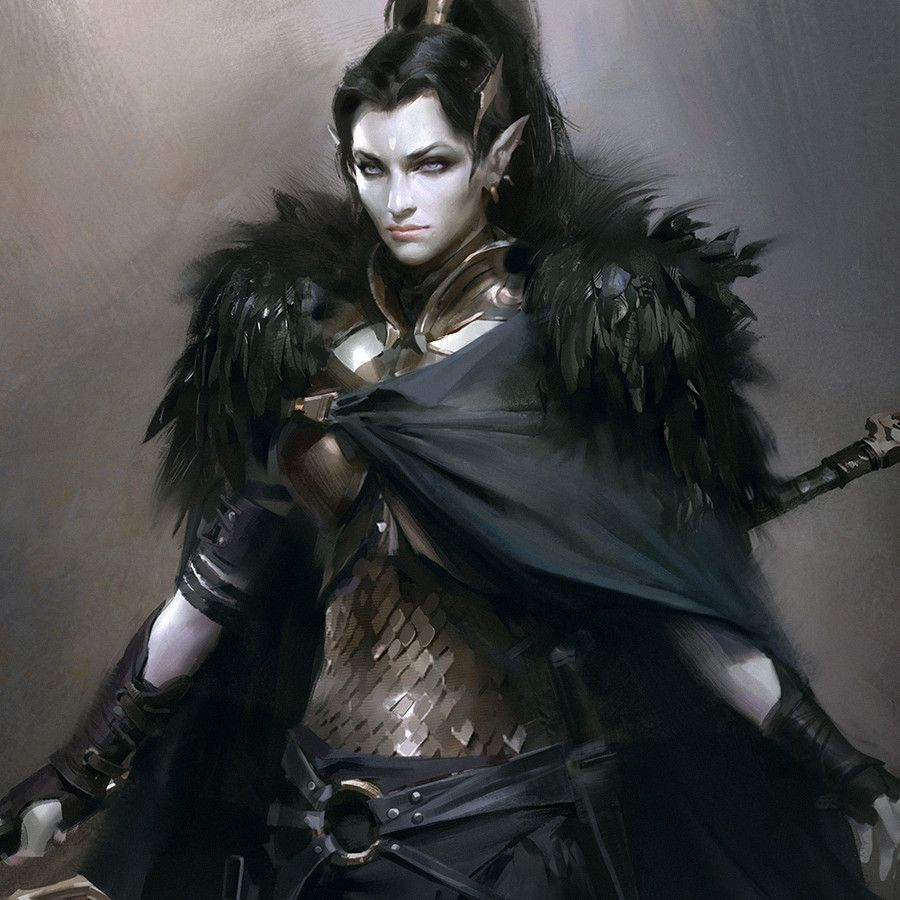
\includegraphics[width=0.6\textwidth]{Nyx.jpg}
    \caption{\label{fig:nyx}Nyx.}
\end{figure}

Nyx, a Shadar-Kai woman, serves as a warrior in the name of the Raven Queen. She possesses a complexion of pale gray skin, striking purple eyes, and cascading,
obsidian black hair. Despite these unique features, she embodies the essence of a typical elven woman.

She adorns herself in the attire of a warrior, donning chain mail and wielding a pike as her weapon of choice. For her journeys, Nyx prefers the practicality
of raven-black cloaks and leather trousers.

Her appearance conveys the image of a formidable fighter, a veteran of numerous battles against the vilest of creatures. Nyx is not known for her overt
friendliness, but those who demonstrate their mettle will earn her trust and respect. To her, the utmost priority lies in accomplishing missions through the
most honorable means possible.

\section{Background}

Born into a family of soldiers, Nyx was raised from a young age as a warrior. She grew up without any siblings. Tragedy struck when she began her military
training, as her parents lost their lives in a devastating battle, marking the most significant loss in the history of their race.

Following the loss of her parents, Nyx dedicated herself tirelessly to her duties and eventually ascended to a high-ranking position within the military. She
emerged as one of her nation's most trusted individuals, and her accomplishments included successfully carrying out missions on behalf of the Raven Queen
herself.

On a particular day, Nyx was entrusted with a critical mission to safeguard an important individual possessing crucial information about their adversaries.
However, on that fateful night, for inexplicable reasons, she drifted into slumber, and tragically, the informant met his demise. Upon awakening, she
discovered the lifeless body of the man. Bewildered by how she had fallen asleep, she soon found herself abandoned by her comrades.

Following that ill-fated incident, Nyx embarked on a journey of exploration and adventure. Leveraging her military background, she willingly undertook diverse
missions and quests. While her primary objective was to reclaim her honor, her path led her to pursue an array of adventures alongside various companions, each
experience adding another layer to her quest for redemption.

\end{document}